% mnras_template.tex
%
% LaTeX template for creating an MNRAS paper
%
% v3.0 released 14 May 2015
% (version numbers match those of mnras.cls)
%
% Copyright (C) Royal Astronomical Society 2015
% Authors:
% Keith T. Smith (Royal Astronomical Society)

% Change log
%
% v3.0 May 2015
%    Renamed to match the new package name
%    Version number matches mnras.cls
%    A few minor tweaks to wording
% v1.0 September 2013
%    Beta testing only - never publicly released
%    First version: a simple (ish) template for creating an MNRAS paper

%%%%%%%%%%%%%%%%%%%%%%%%%%%%%%%%%%%%%%%%%%%%%%%%%%
% Basic setup. Most papers should leave these options alone.
\documentclass[a4paper,fleqn,usenatbib]{mnras}

% MNRAS is set in Times font. If you don't have this installed (most LaTeX
% installations will be fine) or prefer the old Computer Modern fonts, comment
% out the following line
\usepackage{newtxtext,newtxmath}
\usepackage[spanish]{babel}
% Depending on your LaTeX fonts installation, you might get better results with one of these:
%\usepackage{mathptmx}
%\usepackage{txfonts}

% Use vector fonts, so it zooms properly in on-screen viewing software
% Don't change these lines unless you know what you are doing
\usepackage[T1]{fontenc}
\usepackage{ae,aecompl}
\usepackage{float}


%%%%% AUTHORS - PLACE YOUR OWN PACKAGES HERE %%%%%

% Only include extra packages if you really need them. Common packages are:
\usepackage{graphicx}	% Including figure files
\usepackage{amsmath}	% Advanced maths commands
\usepackage{amssymb}	% Extra maths symbols
\usepackage{acronym} % Acronyms
\usepackage{siunitx}

%%%%%%%%%%%%%%%%%%%%%%%%%%%%%%%%%%%%%%%%%%%%%%%%%%

%%%%% AUTHORS - PLACE YOUR OWN COMMANDS HERE %%%%%

% Please keep new commands to a minimum, and use \newcommand not \def to avoid
% overwriting existing commands. Example:
%\newcommand{\pcm}{\,cm$^{-2}$}	% per cm-squared

\acrodef{ATNF}[ATNF]{Australia Telescope National Facility}
\acrodef{PHL}[PHL]{Parkes High-Latitude}
\acrodef{PMB}[PMB]{Parkes Multi-Beam}
\acrodef{SMB}[SMB]{Swinburne Intermediate-latitude}

\acrodef{DSS2}[DSS2]{Digital Sky Survey 2}

%%%%%%%%%%%%%%%%%%%%%%%%%%%%%%%%%%%%%%%%%%%%%%%%%%

%%%%%%%%%%%%%%%%%%% TITLE PAGE %%%%%%%%%%%%%%%%%%%

% Title of the paper, and the short title which is used in the headers.
% Keep the title short and informative.
\title[Short title, max. 45 characters]{Práctica 1 - La Vía Láctea con Gaia}

% The list of authors, and the short list which is used in the headers.
% If you need two or more lines of authors, add an extra line using \newauthor
\author[A. Garcia-Garcia et al.]{
A. Garcia-Garcia$^{1}$\thanks{E-mail: agg180@alu.ua.es}
\\
% List of institutions
$^{1}$Grado en Física, Universidad de Alicante\\
}

% These dates will be filled out by the publisher
\date{}

% Enter the current year, for the copyright statements etc.
\pubyear{2020}

% Don't change these lines
\begin{document}
\label{firstpage}
\pagerange{\pageref{firstpage}--\pageref{lastpage}}
\maketitle

% Abstract of the paper

% Select between one and six entries from the list of approved keywords.
% Don't make up new ones.

%%%%%%%%%%%%%%%%%%%%%%%%%%%%%%%%%%%%%%%%%%%%%%%%%%

%%%%%%%%%%%%%%%%% BODY OF PAPER %%%%%%%%%%%%%%%%%%

\section{Introducción}

En esta práctica trataremos de explorar algunos de los aspectos básicos que intervienen en el estudio de la estructura galáctica. Para ello, nos serviremos principalmente de un catálogo de datos generador por el instrumento astrofísico Gaia: el \emph{Gaia Data Release 2}~\cite{Gaia2018}. Para trabajar con ese catálogo, haremos uso de dos herramientas: el observatorio virtual \emph{Aladin} y la herramienta de procesado y visualización de datos asociada \emph{topcat}.

\section{Ejercicio 1}

\textbf{Selecciona coordenadas galácticas. Consulta la definición de coordenadas galácticas. Toma una región
cercana al centro galáctico ($l=0$, $b=0$), pero no exactamente en esas coordenadas. Carga los datos de
todas las estrellas en una zona circular de radio $10'$. Haz lo mismo para una región completamente alejada
del Plano Galáctico, por ejemplo ($l=180$, $b=-20$). Utiliza diferentes diagramas (por ejemplo, BP-RP/
G, $\pi/G$, etc) para comparar ambas poblaciones. Repite el proceso después de seleccionar solamente aquellos
objetos con errores pequeños en los parámetros astrométricos (e.g. $e_\pi \leq 0.05 ~[mas]$). ¿Qué podemos aprender
(o corroborar de las cosas que se han explicado en clase) a partir de estas poblaciones?}

El sistema de coordenadas galácticas nos permite dar la posición de un objeto en la esfera celeste. Este sistema en particular tiene su centro en el Sol y está alineado con el centro aparente de la Vía Láctea. El plano ecuatorial está alineado con el plano de la galaxia. Las coordenadas pertenecientes a este sistema son longitud $l$ (que se mide sobre el plano en sentido antihorario $0 [\deg] \leq l \leq 360 [\deg]$) y latitud $b$ (que es el ángulo que forma el objeto en cuestión con el plano de la galaxia, siendo positivo al norte y negativo al sur $-90~[\deg] \leq 0 \leq 90~[deg]$).

\begin{figure}
  \includegraphics[width=0.49\linewidth]{img/gaia_2_0}
  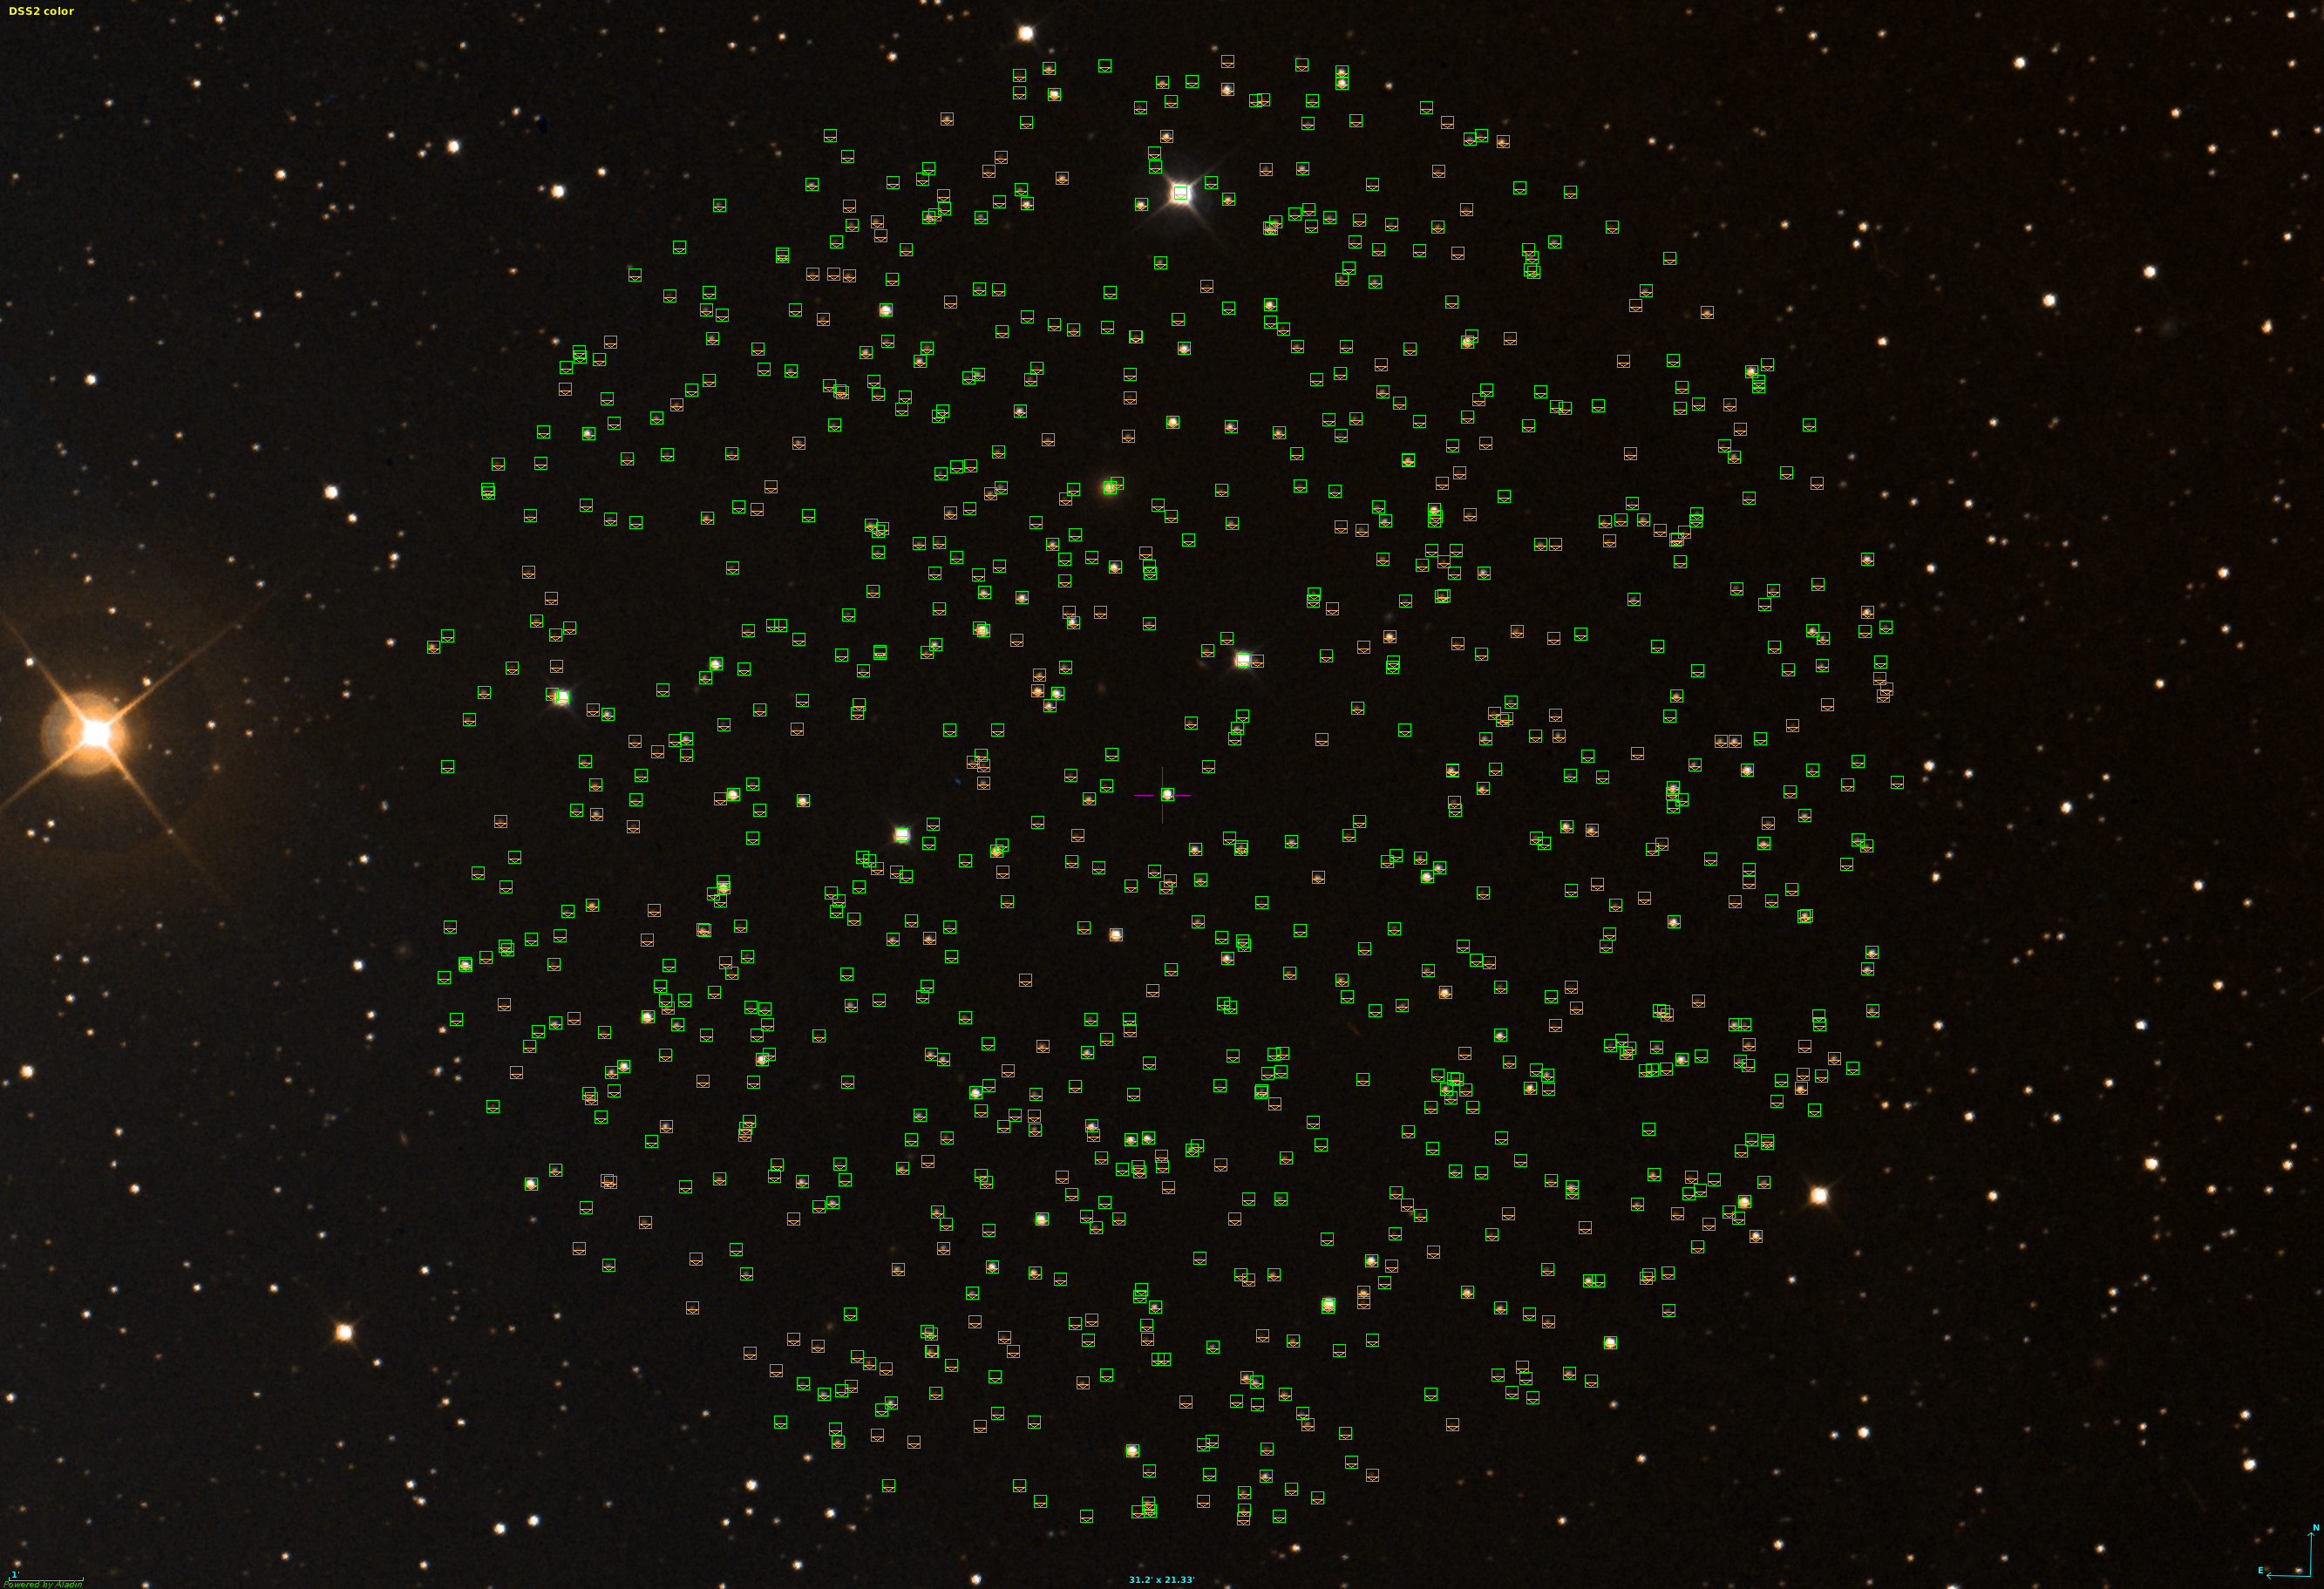
\includegraphics[width=0.49\linewidth]{img/gaia_180_20}
  \caption{Regiones de radio $10'$ de la galaxia seleccionadas para el ejercicio. A la izquierda, imagen de \ac{DSS2} de la región correspondiente a las coordenadas cercanas al plano galáctico $l=2.0,b=0$; a la derecha, región completamente alejada del plano galáctico $l=180,b=-20$. Imágenes obtenidas con el software \emph{Aladin}, las estrellas marcadas con cuadrados verdes corresponden a datos presentes en \emph{Gaia DR2}.}
  \label{fig:e1_regiones}
\end{figure}

Para este primer ejercicio hemos seleccionado dos regiones: la primera de ellas cercana al centro galáctico $(l=2.00, b=0.00)$ y la segunda completamente alejada y anticéntrica $(l=180.00, b=-20.00)$. Empleando el software \emph{Aladin} hemos seleccionado regiones de radio $10'$ centradas en dichas coordenadas y hemos transferido los datos de \emph{Gaia DR2} a \emph{topcat} para su procesado y evaluación. La Figura \ref{fig:e1_regiones} muestra las visualizaciones de \emph{Aladin} para ambas regiones seleccionadas.

Para comparar ambas poblaciones hemos empleado \emph{topcat} para representar diferentes diagramas de las mismas. En primer lugar, visualizaremos el diagrama que previsiblemente más información nos permitirá obtener: un diagrama HR empleando en este caso la fotometría integrada $Gmag$ contra el índice fotométrico azul-rojo $BP-RP$. La Figura \ref{fig:e1_bprpmag} muestra este diagrama.

\begin{figure}
  \includegraphics[width=\linewidth]{img/ejercicio1_bprp_gmag}
  \caption{Diagrama mostrando una representación similar a Hertzsprung-Rusell para las regiones estudiadas pero empleando la fotometría integrada $Gmag$ y el índice fotométrico azul-rojo integrado $BP-RP$ presentes en el catálogo \emph{Gaia DR2}.}
  \label{fig:e1_bprpmag}
\end{figure}

En un diagrama de este estilo podemos apreciar dos efectos principalmente: la distancia de las estrellas (la cual reduce su magnitud aparente y por lo tanto las desplaza hacia abajo en la gráfica) y la extinción (que las enrojece y las desplaza lateralmente a la derecha). El efecto combinado de ambas, desplaza la población diagonalmente hacia la esquina inferior derecha. Atendiendo a estos efectos, la primera comparativa que podemos establecer gracias a este diagrama se puede observar con claridad: la región cercana al centro galáctico posee un efecto mucho más acusado de extinción que la población en el anticentro. Ambas acusan el efecto de la distancia, pero la población en el centro galáctico está mucho más enrojecida. Este efecto es lógico y se debe a la mayor densidad de dicha región y a la mayor presencia de factores en el medio interestelar cercano al centro galáctico.

Por otro lado, podemos comparar las poblaciones atendiendo a otros criterios como el paralaje $Plx$ y su plano de movimientos propios $pmRA$ y $pmDE$. Las Figuras \ref{fig:e1_plx} y \ref{fig:e1_pmrapmde} muestran una comparativa de ambas poblaciones atendiendo a dichos parámetros.

\begin{figure}
  \includegraphics[width=\linewidth]{img/ejercicio1_plx_gmag}
  \caption{Diagrama de paralaje $Plx$ contra magnitud integrada $Gmag$ para las poblaciones seleccionadas con los datos de \emph{Gaia DR2}.}
  \label{fig:e1_plx}
\end{figure}

\begin{figure}
  \includegraphics[width=\linewidth]{img/ejercicio1_pmra_pmde}
  \caption{Diagrama de movimientos propios en ascensión recta $pmRA$ y declinación $pmDE$ para las poblaciones seleccionadas con los datos de \emph{Gaia DR2}.}
  \label{fig:e1_pmrapmde}
\end{figure}

\newpage

De estas dos representaciones se desprende y se corrobora la uniformidad de la galaxia: ambas poblaciones pese a residir en regiones diametralmente opuestas poseen una distribución de paralajes y de movimientos propios muy similar.

Para completar este ejercicio, repetiremos el análisis anterior seleccionando únicamente aquellos objetos con errores pequeños en los parámetros astrométricos. Para realizar este filtrado, emplearemos la herramienta de subconjuntos de \emph{topcat}. Trataremos por lo tanto, de conservar aquellos objetos que residan en el $~10\%$ con menores errores astrométricos para paralaje $ePlx$ y movimientos propios $ePMRA$ y $ePMDE$. En la Figura \ref{fig:e1_eplx} se muestra un filtrado de ejemplo conservando aquellos objetos con un error en paralaje inferior a $0.05~[mas]$.

\begin{figure}
  \includegraphics[width=0.49\linewidth]{img/ejercicio1_eplx}
  \includegraphics[width=0.49\linewidth]{img/ejercicio1_eplx_filtered}
  \caption{Gráfica de error en paralaje $ePlx$ contra $Gmag$ (izquierda) y la misma gráfica pero con todos aquellos objetos con error mayor que $0.05$ filtrados.}
  \label{fig:e1_eplx}
\end{figure}

En las Figuras \ref{fig:e1_bprpmag_filtered}, \ref{fig:e1_plx_filtered} y \ref{fig:e1_pmrapmde_filtered} se muestran los diagramas HR, paralaje contra magnitud y plano de movimientos propios respectivamente, esta vez omitiendo aquellos objetos con errores por encima de los umbrales comentados en los parámetros astrométricos.

\begin{figure}
  \includegraphics[width=\linewidth]{img/ejercicio1_bprp_gmag_filtered}
  \caption{Diagrama mostrando una representación similar a Hertzsprung-Rusell para las regiones estudiadas pero empleando la fotometría integrada $Gmag$ y el índice fotométrico azul-rojo integrado $BP-RP$ presentes en el catálogo \emph{Gaia DR2}. Se muestran únicamente los objetos con errores astrométricos reducidos.}
  \label{fig:e1_bprpmag_filtered}
\end{figure}

\begin{figure}
  \includegraphics[width=\linewidth]{img/ejercicio1_plx_gmag_filtered}
  \caption{Diagrama de paralaje $Plx$ contra magnitud integrada $Gmag$ para las poblaciones seleccionadas con los datos de \emph{Gaia DR2}. Se muestran únicamente los objetos con errores astrométricos reducidos.}
  \label{fig:e1_plx_filtered}
\end{figure}

\begin{figure}
  \includegraphics[width=\linewidth]{img/ejercicio1_pmra_pmde_filtered}
  \caption{Diagrama de movimientos propios en ascensión recta $pmRA$ y declinación $pmDE$ para las poblaciones seleccionadas con los datos de \emph{Gaia DR2}. Se muestran únicamente los objetos con errores astrométricos reducidos.}
  \label{fig:e1_pmrapmde_filtered}
\end{figure}

\newpage

Al aplicar este filtrado, el efecto más notable que apreciamos es la eliminación de todas aquellas estrellas de magnitud por encima de $16$ aproximadamente. Es lógico pensar que para estrellas tan poco brillantes estén sujetas a un error mayor dados los márgenes de sensibilidad de la instrumentación astrofísica. Si descartamos aquellos datos con mayor incertidumbre, ambas poblaciones siguen teniendo una situación en el plano de movimientos propios y una distribución de paralajes similar. Al descartar también aquellas estrellas más distantes y por lo tanto más afectadas por la extinción, el diagrama HR se torna más similar para las dos poblaciones.

Para finalizar este ejercicio, podemos reflexionar sobre aquellos hechos explicados en clase que podemos corroborar a partir de las dos poblaciones: (1) la distribución de la galaxia, desde nuestro punto de vista, es prácticamente homogénea (ambas poblaciones presentan características muy similares), (2) la poca fiabilidad de los instrumentos para objetos de poco brillo (hemos observado cómo los objetos con magnitud fotométrica integrada a partir de 16 presentan una tasa de error muy elevada), (3) el efecto notable de la distancia y la extinción (tal y como hemos observado en los diagramas HR, las estrellas más lejanas se ven afectadas en gran medida por la extinción en aquellas zonas de mayor densidad de objetos).

\section{Ejercicio 2}

\textbf{Carga los datos para las estrellas en torno al cúmulo abierto de las Pléyades (M45). Este es un cúmulo muy cercano. Necesitarás tomar un radio grande (de, por lo menos, un grado). Intenta localizar el cúmulo en el plano de los movimientos propios. Estudia su extensión en diferentes diagramas y selecciona un conjunto de posibles miembros del cúmulo. Haz el mismo estudio para el cúmulo abierto problema que se ha asignado a tu grupo. Este cúmulo es más lejano y necesitarás tomar un radio entre $10'$ y $20'$. Una vez tengas una selección de miembros, identifica las estrellas evolucionadas que pertenecen al cúmulo. Dibuja el diagrama color/magnitud (en este caso, BP-RP/G) para los dos cúmulos. ¿Qué diferencias ves? ¿A qué puedes atribuirlo?}

Para este segundo ejercicio hemos empleado \emph{Aladin} para seleccionar una región de radio $60'$ en las coordenadas galácticas del cúmulo M45 ($l=166.57, b=-23.522$). En la Figura \ref{fig:e2_m45} mostramos la visualización de dicho cúmulo así como los datos de \emph{Gaia DR2} que serán transmitidos a \emph{topcat} para su posterior análisis.

\begin{figure}
  \centering
  \includegraphics[width=0.75\linewidth]{img/pleyades}
  \includegraphics[width=0.75\linewidth]{img/pleyades_gaia}
  \caption{Región de $60'$ (1 grado) respecto al centro del cúmulo M45. A la izquierda, datos del catálogo \ac{DSS2} centrados en las coordenadas $l=166.56979, b=-23.52246$; a la derecha, la misma imagen con los datos de \emph{Gaia DR2} sobreimpuestos como cuadrados turquesas en la región dada. Imágenes obtenidas con el software \emph{Aladin}.}
  \label{fig:e2_m45}
\end{figure}

Como podemos observar, en dicha región hemos seleccionado una gran cantidad de estrellas que no pertenecen al cúmulo en sí. A continuación procederemos a intentar localizar el cúmulo verdadero mediante la visualización de los datos astrométricos de la población inicial.

En primer lugar, podemos realizar un primer filtrado eliminando todos aquellos objetos cuya magnitud exceda 14 (para los cuales de cualquier manera las medidas de las que disponemos poseen errores bastante elevados). En la Figura \ref{fig:e2_bprpgmag} se muestra el diagrama HR y el mismo filtrado de acuerdo a este criterio.

\begin{figure}
  \includegraphics[width=0.49\linewidth]{img/ejercicio2_m45_bprp_gmag}
  \includegraphics[width=0.49\linewidth]{img/ejercicio2_m45_bprp_gmag_14}
  \caption{Diagramas HR (en nuestro caso $Gmag$ contra $BP-RP$) para el cúmulo M45. A la izquierda, el diagrama completo. A la derecha, el mismo diagrama pero filtrando las estrellas de magnitud por encima de 14.}
  \label{fig:e2_bprpgmag}
\end{figure}

Seguidamente, procederemos a analizar los movimientos propios. En la Figura \ref{fig:e2_pmrapmde} podemos observar el diagrama del plano de movimientos propios $pmRA$ y $pmDE$ en el que apreciamos dos grupos claramente diferenciados (además del prefiltrado por magnitud). Asumiendo que las estrellas del cúmulo han de tener movimientos propios similares, nuestro cúmulo se encuentra en uno de estos dos candidatos.

\begin{figure}
  \includegraphics[width=\linewidth]{img/ejercicio2_m45_pmde_pmra_14}
  \caption{Diagrama de movimientos propios en ascensión recta y declinación para el cúmulo M45 mostrando dos posibles candidatos (clústers) de objetos. También se muestra el resultado de realizar el filtrado por magnitud antes mencionado (en amarillo).}
  \label{fig:e2_pmrapmde}
\end{figure}

Si representamos el paralaje $Plx$ podemos distinguir y refinar aún mejor los dos cúmulos tal y como se muestra en la Figura \ref{fig:e2_plx}. Aplicando el mismo procedimiento, podemos representar el movimiento propio contra el paralaje en declinación o ascensión recta tal y como vemos en la Figura \ref{fig:e2_pmde} y obtener así un cúmulo todavía más refinado. Dado que nos enfrentamos a un cúmulo relativamente reducido, asumiremos que el subconjunto más pequeño de los obtenidos es el que verdaderamente representa al cúmulo M45 buscado.

\begin{figure}
  \includegraphics[width=\linewidth]{img/ejercicio2_m45_plx_pmra}
  \caption{Diagrama de movimiento propio $RA$ contra paralaje $Plx$. Un nuevo clúster (azul) es diferenciado respecto al subconjunto anterior.}
  \label{fig:e2_plx}
\end{figure}

\begin{figure}
  \includegraphics[width=\linewidth]{img/ejercicio2_m45_plx_pmde}
  \caption{Diagrama de movimiento propio $DE$ contra paralaje $Plx$. Otro nuevo clúster (verde) puede ser diferenciado incluido en el subconjunto anterior.}
  \label{fig:e2_pmde}
\end{figure}

Si transportamos estos datos refinados de vuelta al observatorio virtual \emph{Aladin}, tal y como se muestra en la Figura \ref{fig:e2_final_m45}, podemos comprobar que hemos identificado las estrellas del cúmulo con efectividad.

\begin{figure}
  \includegraphics[width=\linewidth]{img/m45_cumulo_def}
  \caption{Resultados del cúmulo identificado visualizado de nuevo en \emph{Aladin}. Los datos originales transferidos a \emph{topcat} están marcados como círculos rojos mientras que el cúmulo seleccionado finalmente está indicado con rectángulos verdes.}
  \label{fig:e2_final_m45}
\end{figure}

A continuación, realizaremos el mismo estudio para el cúmulo problema \emph{Berkeley 51}. De la misma forma que antes, hemos empleado \emph{Aladin} para seleccionar una región de radio $10'$ en las coordenadas galácticas del cúmulo \emph{Berkeley 51}. La Figura \ref{fig:e2_b51} muestra dicho cúmulo en \emph{Aladin}. En la bibliografía proporcionada por \emph{Simbad}\footnote{http://simbad.u-strasbg.fr/simbad/sim-id?Ident=C2010\%2B342} sobre este cúmulo podemos encontrar una serie de referencias de gran relevancia: \cite{Negueruela2018,Lohr2018,Tadross2008,Ruprecth1966}.

De dicha bibliografía podemos extraer una gran cantidad de información de alto nivel sobre el cúmulo a estudiar:

\begin{itemize}
  \item Se trata de un cúmulo abierto joven y altamente enrojecido. 
  \item Se han identificado cuatro y cinco supergigantes amarillas y rojas respectivamente (tipos espectrales de F a M).
  \item Dos de las supergigantes amarillas muestran cierta variedad espectral (tipo F8 Ib y comportamiento típico de cefeidas).
  \item La distancia estimada es de $5.5~[kpc]$, obtenida mediante un ajuste a la secuencia principal.
  \item Se sugiere una edad de aproximadamente $60~[Ma]$ por ajuste isócrono.
  \item Cerca del centro del cúmulo encontramos una supergigante de tipo M2 Iab.
  \item Posee una candidata importante a cefeida BE51\#162.
\end{itemize}

\begin{figure}
  \centering
  \includegraphics[width=\linewidth]{img/cumulo_berkeley}
  \includegraphics[width=\linewidth]{img/cumulo_berkeley_gaia}
  \caption{Región de $4'$ respecto al centro del cúmulo Berkeley 51. Arriba, datos del catálogo \ac{DSS2} centrados en las coordenadas $l=72.1536, b=00.2964$; abajo, la misma imagen con los datos de \emph{Gaia DR2} sobreimpuestos como círculos verdes en la región dada. Imágenes obtenidas con el software \emph{Aladin}.}
  \label{fig:e2_b51}
\end{figure}

Cabe destacar que, atendiendo a \cite{Tadross2008}, el cúmulo posee un diámetro de $2'$. En nuestro estudio hemos escogido un diámetro algo más grande de $4'$ con el objetivo de comprobar si somos capaces de aislar las estrellas del cúmulo mediante el estudio de los diversos diagramas. Algunas de ellas obvias y otras no tan sencillas de distinguir. A continuación, procederemos a la visualización de los datos astrométricos con \emph{topcat} y, atendiendo también a las características básicas del cúmulo obtenidas en la bibliografía, trataremos de obtener el conjunto de estrellas que verdaderamente pertenecen a Berkeley 51.

En primer lugar, en la Figura \ref{fig:e2_b51} podemos visualizar el diagrama HR (en nuestro caso BP-RP / Gmag). Realizaremos un corte para aquellos objetos con un alto error en sus magnitudes astrométricas. Tras visualizar la evolución de dichos errores, hemos considerado que la magnitud 18 es un buen límite para filtrar la calidad de los datos.

\begin{figure}
  \includegraphics[width=\linewidth]{img/b51_bprp_gmag}
  \caption{Diagrama HR (en nuestro caso $Gmag$ contra $BP-RP$) para el cúmulo B51. Mostramos (en rojo) todos los objetos seleccionados y los objetos filtrados quedándonos con aquellos que posean bajas cotas de error en sus parámetros astrométricos (en azul).}
  \label{fig:e2_b51_bprpgmag}
\end{figure}

Seguidamente, visualizaremos otra vista que nos permita diferenciar las estrellas evolucionadas del cúmulo respecto al resto no pertenecientes al mismo: el plano de los movimientos propios. Las Figuras \ref{fig:e2_b51_pmrapmde} y \ref{fig:e2_b51_radec} muestran el diagrama de movimientos propios (pmRA vs. pmDE) para los objetos anteriormente seleccionados y para el subconjunto trazado atendiendo a este propio diagrama respectivamente (bajo la hipótesis de que las estrellas evolucionadas del cúmulo han de tener movimientos propios similares o por lo menos no enormemente dispares).

\begin{figure}
  \includegraphics[width=\linewidth]{img/b51_pmra_pmde}
  \caption{Diagrama de movimientos propios en ascensión recta y declinación para el cúmulo B51 mostrando dos posibles candidatos (clústers) de objetos: tanto todos los objetos seleccionados en \emph{Aladin} (rojo) como aquellos filtrados por magnitud (azul).}
  \label{fig:e2_b51_pmrapmde}
\end{figure}

\begin{figure}
  \includegraphics[width=\linewidth]{img/b51_radec}
  \caption{Diagrama de movimientos propios en ascensión recta y declinación para el cúmulo M51 mostrando tres posibles candidatos de clústers: (rojo) los objetos originales, (azul) objetos filtrados por magnitud y (verde) subconjunto seleccionado con movimientos propios similares.}
  \label{fig:e2_b51_radec}
\end{figure}

Por último, para poder trazar una distinción más crítica, visualizaremos el diagrama de movimiento propio en ascensión recta contra paralaje en la Figura \ref{fig:e2_b51_plx}. En dicho diagrama hemos seleccionado otro subconjunto con paralaje y movimiento propio en ascensión recta similar.

\begin{figure}
  \includegraphics[width=\linewidth]{img/b51_plx}
  \caption{Diagrama de movimiento propio $RA$ contra paralaje $Plx$. Un nuevo clúster (gris) es diferenciado respecto al subconjunto anterior.}
  \label{fig:e2_b51_plx}
\end{figure}

Después de todo este filtrado, podemos tener una mejor idea de las estrellas evolucionadas que forman parte verdaderamente del cúmulo. Como podemos comprobar en la Figura \ref{fig:e2_b51_aladin}, si transferimos estos datos de vuelta a \emph{Aladin}, hemos sido capaces de identificar correctamente la mayor parte de estrellas enrojecidas y evolucionadas pertenecientes al cúmulo mientras que hemos dejado fuera todas aquellas de tipos espectrales diferentes y menos enrojecidas que presumiblemente no pertenecen al cúmulo objetivo.

Las estrellas identificadas y pertenecientes al cúmulo se muestran en la Tabla \ref{table:b51} junto con sus identificadores en los catálogos correspondientes y sus coordenadas.

Por otro lado, en la Figura \ref{fig:e2_m45_b51} podemos observar una comparativa de los diagramas HR tanto para los datos seleccionados en el cúmulo M45 como para el cúmulo objetivo Berkeley51. De dicha figura podemos extraer varias conclusiones:

\begin{itemize}
  \item Efectivamente, el cúmulo B51 está desplazado a la derecha respecto al M45 y por lo tanto mucho más enrojecido.
  \item El cúmulo B51 está mucho más afectado por la distancia que el cúmulo M45 (desplazamiento vertical y extinción). Atendiendo a los datos, de hecho, el cúmulo M45 es ciertamente mucho más cercano.
  \item Observamos también la presencia de supergigantes rojas y amarillas en el caso de B51 pero no en M45 (en el cual la mayoría de las estrellas están en secuencia principal).
  \item Observamos la presencia de posibles enanas blancas en el diagrama HR de M45, no así en el caso de B51.
  \item En general, el cúmulo M45 está mucho más poblado que el cúmulo B51.
\end{itemize}

\newpage

\begin{figure}
  \includegraphics[width=\linewidth]{img/b51_aladin}
  \caption{Resultados del cúmulo identificado visualizado de nuevo en \emph{Aladin}. Los datos originales transferidos a \emph{topcat} están marcados como círculos rojos mientras que el cúmulo seleccionado finalmente está indicado con rectángulos verdes.}
  \label{fig:e2_b51_aladin}
\end{figure}


\begin{table}
  \caption{Lista de estrellas en el cúmulo Berkeley 51 extraída de la herramienta \emph{Simbad}.}
  \resizebox{\linewidth}{!}{
  \begin{tabular}{c|c|c}
  \# & Catálogo e Identificador & Coordenadas (ICRS,J2000/2000) \\
  \hline
  1  & 2MASS J20115005+3425028      & 20 11 50.0546321696 +34 25 02.749686434 \\
  2  & 2MASS J20115645+3424222      & 20 11 56.4411840807 +34 24 22.206964366 \\
  3  & Gaia DR2 2055722466316862976 & 20 12 03.7217196755 +34 25 04.559180572 \\
  4  & Gaia DR2 2055722535028287104 & 20 11 53.9483574818 +34 23 54.591310474 \\
  5  & Gaia DR2 2055718922944280192 & 20 11 58.8788001990 +34 21 09.622910962 \\
  6  & Gaia DR2 2055722225798781696 & 20 11 49.3970985794 +34 24 09.742825064 \\
  7  & Gaia DR2 2055722191439041408 & 20 11 47.4750152119 +34 23 22.422433551 \\
  8  & Gaia DR2 2055722328869693440 & 20 11 59.6027695781 +34 23 22.392957036 \\
  9  & Gaia DR2 2055719305220885632 & 20 12 03.2966417461 +34 22 24.266511463 \\
  10 & Gaia DR2 2055722431957076352 & 20 12 08.6536643358 +34 24 12.173629896 \\
  11 & Gaia DR2 2055722981713031424 & 20 11 48.2014477078 +34 24 04.265982196 \\
  12 & Gaia DR2 2055722393277929088 & 20 12 05.8501494573 +34 24 10.465235085 \\
  13 & Gaia DR2 2055722530716877184 & 20 11 55.7969643369 +34 23 47.113290563 \\
  14 & Gaia DR2 2055722461997415296 & 20 12 05.2314411590 +34 24 29.816149172 \\
  15 & Gaia DR2 2055722530716886144 & 20 11 56.1271635432 +34 24 04.112607580 \\
  16 & Gaia DR2 2055722603755888256 & 20 11 51.7806251786 +34 24 18.541681979 \\
  17 & Gaia DR2 2055722603755884672 & 20 11 53.6337739553 +34 24 47.350277107 \\
  18 & Gaia DR2 2055723428389662848 & 20 11 47.2337793263 +34 25 27.182649079 \\
  19 & Gaia DR2 2055722535028295424 & 20 11 53.9665853664 +34 24 04.450662316 \\
  20 & Gaia DR2 2055722221479222912 & 20 11 50.7581702549 +34 23 33.697276471 \\
  21 & Gaia DR2 2055722187119477376 & 20 11 49.6900784087 +34 23 16.598636830 \\
  22 & Gaia DR2 2055722535036372864 & 20 11 56.5953786228 +34 24 14.603770161 \\
  23 & Gaia DR2 2055722530716872576 & 20 11 56.5376221479 +34 23 41.751631412 \\
  24 & Gaia DR2 2055722535036380160 & 20 11 55.9257236632 +34 24 21.049076259 \\
  25 & Gaia DR2 2055723050432539392 & 20 11 46.5562753237 +34 25 08.145797140 \\
  \end{tabular}}
  \label{table:b51}
\end{table}

\begin{figure}
  \includegraphics[width=0.5\linewidth]{img/m45_b51_1}
  \includegraphics[width=0.5\linewidth]{img/m45_b51_2}
  \caption{Comparativa de diagramas HR (BP-RP / Gmag) de los objetos seleccionados para el cúmulo M45 (izquierda) y para el cúmulo objetivo Berkeley51 (derecha).}
  \label{fig:e2_m45_b51}
\end{figure}

\section{Ejercicio Opcional}

\textbf{Para las estrellas evolucionadas del cúmulo problema descarga datos fotométricos de diferentes catálogos y estudia su distribución espectral de energía. ¿Qué te puede ser necesario?}

En la Figura \ref{fig:e2_b51_simbad} podemos observar aquellas estrellas evolucionadas del cúmulo para las que poseemos datos de \emph{Simbad} y por lo tanto están identificadas (son las estrellas, o mejor dicho, el subconjunto de ellas de las que identificamos en el ejercicio anterior como candidatas del cúmulo).

\newpage

Empleando los datos de \emph{Gaia}, en concreto la temperatura efectiva Teff, podemos generar un pseudo-diagrama de distribución espectral como se muestra en la Figura \ref{fig:e2_b51_teff}. En él, podemos confirmar que la mayor parte de las estrellas del cúmulo son de tipo M ($2500-3500~[K]$) o K ($3500-5000~[K]$) y algunas G ($5000-6000~[K]$) y F ($6000-7500~[K]$).

\begin{figure}
  \includegraphics[width=\linewidth]{img/simbad_b51}
  \caption{Estrellas identificadas por \emph{Simbad} (en rojo) en el cúmulo Berkeley 51 y aquellas para las que disponemos de datos de Gaia (en azul).}
  \label{fig:e2_b51_simbad}
\end{figure}

\begin{figure}
  \includegraphics[width=\linewidth]{img/b51_teff}
  \caption{Histograma de distribución de temperatura de las estrellas del cúmulo Berkeley 51.}
  \label{fig:e2_b51_teff}
\end{figure}

\section{Conclusión}

En esta práctica hemos empleado las herramientas \emph{Simbad} y \emph{topcat} tanto para analizar poblaciones de estrellas en regiones dispares de la galaxia como para tratar de identificar aquellas pertenecientes a ciertos cúmulos aislándolas de otras poblaciones de estrellas fuera de ellos. Esto nos ha permitido reforzar los conocimientos aprendidos sobre la galaxia así como aprender a discernir información de cúmulos a partir de los datos astrométricos.


%%%%%%%%%%%%%%%%%%%%%%%%%%%%%%%%%%%%%%%%%%%%%%%%%%

%%%%%%%%%%%%%%%%%%%% REFERENCES %%%%%%%%%%%%%%%%%%

% The best way to enter references is to use BibTeX:

\bibliographystyle{mnras}
\bibliography{mnras} % if your bibtex file is called example.bib


%%%%%%%%%%%%%%%%%%%%%%%%%%%%%%%%%%%%%%%%%%%%%%%%%%

%%%%%%%%%%%%%%%%% APPENDICES %%%%%%%%%%%%%%%%%%%%%


%%%%%%%%%%%%%%%%%%%%%%%%%%%%%%%%%%%%%%%%%%%%%%%%%%


% Don't change these lines
\bsp	% typesetting comment
\label{lastpage}
\end{document}

% End of mnras_template.tex